%*******************************************************************************
% Copyright (c) 2014 Formal Mind GmbH and others
% All rights reserved. This program and the accompanying materials
% are made available under the terms of the Eclipse Public License v1.0
% which accompanies this distribution, and is available at
% http://www.eclipse.org/legal/epl-v10.html
% 
% Contributors:
%     Michael Jastram - initial Copy
%     Maha Jastram - susequent improvements
%******************************************************************************/

% ===================================================================================
\section{Eclipse}
\label{sec:eclipse}
% ===================================================================================

\pror{} is an extension of the generic Eclipse Platform.  The following is concerned with Eclipse in general.

\begin{info}
Please consult the 
\eclipsehelp{/topic/org.eclipse.platform.doc.user/gettingStarted/intro/overview.htm?cp=0_0}{Eclipse platform overview} for further information.
\end{info}

% -----------------------------------------------------------------------------------
\subsection{Prerequisites}
% -----------------------------------------------------------------------------------

Eclipse is a Java-based application.  You need a Java Runtime Environment (JRE) on your computer in order to run \pror{}.

\pror{} requires JRE 1.6 or better.  However, some of the features from Essentials require JRE 1.7 or better.  Further, we recommend the version from Oracle, and not OpenJDK.

\begin{info}
You can download Java at \href{https://www.java.com}{java.com}.
\end{info}

% -----------------------------------------------------------------------------------
\subsection{Installation}
\label{sec:installation}
\index{installation}
% -----------------------------------------------------------------------------------

This chapter explores the installation of \term{Eclipse Products}, i.e. software that you can download and run on your computer.  This is in contrast to \term{features} or \term{plugins}, which can be added to an existing product.

When working with Eclipse, you have to start with a base installation.  However, we recommend using \href{https://reqif.academy}{ReqIF Studio}, but you can start with any Eclipse product.

Once you have identified the product you would like to use, you need to download it, which is typically a .zip file.  Create a folder and extract the content of the .zip file into that folder.

\begin{info}
We recommend to call the folder \menu{studio} and to store it where your executables are located: On Windows in \menu{Program Files}, on Linux in \menu{~/bin}.  But any location will do.

We recommend to creating a shortcut for launching it.
\end{info}

You launch the product by double-clicking on the launcher in the folder you created.  For \pror{}, this is called \menu{studio.exe} or \menu{studio}.

The first time you launch Eclipse, it will ask you for the \term{Workspace} location, see Section \ref{sec:workspaces}.

% -----------------------------------------------------------------------------------
\subsection{Updates}
\label{sec:update}
\index{updating}
\index{updates}
% -----------------------------------------------------------------------------------

The Eclipse Update Manager regularly checks for new versions and alerts the user if one is found.  It can also be started manually via \menu{Help | Check for Updates}.

% -----------------------------------------------------------------------------------
\subsection{Installing New Features}
\label{sec:install-add-on}
% -----------------------------------------------------------------------------------

Before you start installing new features, you typically need to connect with the update site that is hosting the feature to be installed.

\begin{definition}{Update Site}
\index{update site}
An update site is a machine-readable URL that allows \pror{} to install new functionality.  Note that visiting the update site with a web browser rarely produces anything meaningful.
\end{definition}

To install a new feature, follow these steps:

\begin{itemize}
\item Open the installation dialog via \menu{Help | Install new Software...}.
\item In the \menu{Work with:} dropbox, either paste the Update Site URL, or select it from the drop down, if you have used it before.  Note that some popular update site URLs may already be preinstalled.
\item Upon selecting an update site, you will see a list of components available from that update site.  Note the checkboxes below that may result in some entries being hidden.  In particular, some update sites do not categorize.  Unchecking \menu{Group items by category} may unveil hidden entries.
\item Click \menu{Next >}.  If all dependencies can be resolved, details about the installation are shown.  Otherwise you have to troubleshoot dependencies (an unthankful job!).
\item Click \menu{Next >}, review and accept the license.
\item Click \menu{Finish}.  If the component has not been digitally signed, you will receive a warning, which you can typically ignore.
\item It is recommended to restart after the installation.
\end{itemize}

\index{unsigned content}
\index{signed content}
\begin{info}
\textbf{Signatures on Content.}  In this day and age, security is obviously very important, particularly for content downloaded from the Internet.  But note that signing is not enough: content must be signed with a trusted, non-expired signature.

Eclipse content should be signed by eclipse.org.  Especially small project release plug-ins that are not signed, reasoning that to a user, a self-signed signature is as good (or bad) as a missing signature.

Ultimately, you need to decide for yourself whether you are willing to run unsigned and/or untrusted content.
\end{info}

% -----------------------------------------------------------------------------------
\subsection{Workspaces}
\label{sec:workspaces}
% -----------------------------------------------------------------------------------

The workspace is a folder on your computer, where all information related to \pror{} is stored.  This includes all your ReqIF files, organized into projects, as well as various meta data.

\begin{info}
Read more about the \eclipsehelp{/topic/org.eclipse.platform.doc.user/gettingStarted/qs-02a.htm?cp=0_1_0_0}{The Workbench} in the Eclipse documentation.

Also, it is possible to have more than one workspace, and to switch between them.  This feature can be useful for advanced users.
\end{info}

% -----------------------------------------------------------------------------------
\subsection{Committer License Agreement (CLA)}\index{Committer License Agreement}
% -----------------------------------------------------------------------------------

The Committer License Agreement (CLA) needs to be signed by contributors to Eclipse projects.  It essentially states that you hold all rights to your contribution and that you allow Eclipse to use them under the Eclipse Public License.

% ===================================================================================
\section{\pror{} User Interface}
\index{user interface}
\index{main window}
% ===================================================================================

Figure~\ref{fig:user_interface_overview} shows the user interface of \pror{}.

\begin{figure}
  \centering
  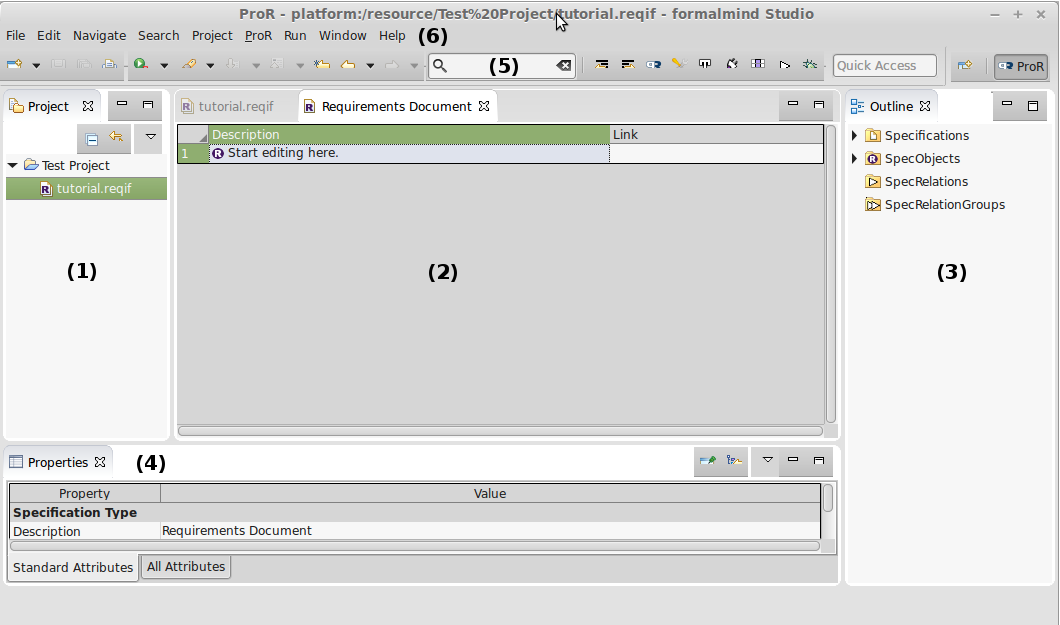
\includegraphics[width=\linewidth]{../rmf-images/Screenshot_intro.png}
  \caption{The \pror{} user interface}
  \label{fig:user_interface_overview}
\end{figure}

\paragraph{(1)} The \menu{Project Explorer} shows a hierarchical listing of the project and the associated models.

\paragraph{(2)} The editor area shows two kinds of editors.  First, each ReqIF file has a \menu{ReqIF Editor} that shows basic information about the mode.  In addition, \menu{Specification Editors} can be opened for each Specification.

\paragraph{(3)} The \menu{Outline View} has four folders that show the content of the selected model:

\begin{description}

\item[Specifications] shows the Specifications in the ReqIF model.  You can
  expand the tree to expose the hierarchy of SpecObjects in each Specification.
\item[SpecObjects] shows all SpecObjects in the ReqIF model as a flat list.
  Keep in mind that SpecObjects in Specifications are references.  In
  contrast, this folder shows all SpecObjects created for the ReqIF model, whether or not they are referenced.
\item[SpecRelations] shows all SpecRelations in the ReqIF as a flat list.
\item[SpecRelationsGroups] represents an optional mechanism for grouping SpecRelations between two specific specifications.
\end{description}

\paragraph{(4)} The properties of a selected Element are shown in the \menu{Properties View}.  It has two tabs, one for \menu{Standard Attributes} and one for \menu{All Attributes}.

\paragraph{(5)} Above the main working windows is the tool bar, which may change according to which editor is active.

\paragraph{(6)} The menu bar provides access to all Eclipse and \pror{} features.

% -----------------------------------------------------------------------------------
\subsection{Editors and Views}
\label{sec:editorsviews}
\index{editor}
\index{view}
% -----------------------------------------------------------------------------------

The Eclipse user interface consists of \term{Views} and \term{Editors}.  Views change their content according to the current selection and are not savable.  Editors are typically associated with a resource (e.g. a file) and can be saved.  The editors' selection can determine what is shown in the Views.  For instance, the \menu{Properties View} typically shows details about the element selected in the \menu{Specification Editor}.

You can browse through the available Views and open them via \menu{Window | Show Views...}, resulting in a menu similar to the one shown in Figure~\ref{fig:Views}.

\begin{figure}
\centering
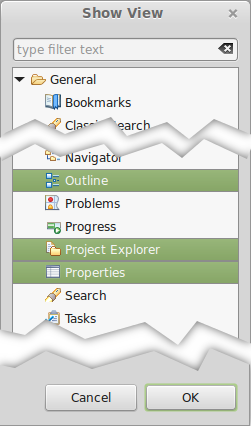
\includegraphics[width=.3\textwidth]{../rmf-images/views_highlighted.png}
\caption{Views.}
\label{fig:Views}
\end{figure}

Upon opening a ReqIF model, the editor opens providing an overview of the model.  In essence what you are seeing is the Eclipse Workbench, with several modifications.  Here you will find a quick overview of each component.  A more detailed description of the Workbench can be found in 
\eclipsehelp{org.eclipse.platform.doc.user/reference/ref-43.htm}{Eclipse's Workbench User Guide}.

\begin{info}
  There may be more than one editor for a given file type.  To pick a specific one, right-click the file and select \menu{Open With...}, which will give you the list of installed editors.  In particular, the \menu{fmStudio Main Editor} from Formal Mind is more powerful than the stock editor (see Section~\ref{sec:StudioSpecEditor}).
\end{info}

A model contains any number of Specifications, and the details of each Specification can be inspected individually.  The windows in which all relevant information appears are called \term{views}.  At your disposal are many views with productivity, debugging, help and team resources.  We will be focusing only on the views relevant to \pror{}.


